\section{\textcolor[HTML]{D32F2F}{Papirprototyping}}
% For å finne et design som passet kundenes behov, ble det valgt å følge en iterativ prosess. Dette er nyttig når man skal utvikle et produkt for en brukergruppe, fordi man underveis kan endre og tilpasse til kundenes behov. En iterativ prosess består gjerne av fire faser; analyse, design, prototype og testing\cite{brukersentrert}. I første runde kan prototypene være svært primitive, low-fidelity, som for eksempel en papirprototype. Senere i prosessen kan man med fordel gjøre prototypen med avansert, for eksempel ved å lage en high-fidelity prototype\cite{paperprototype}.
\\\\
Da gruppen skulle begynne å designe produktet var det noen ting som var viktige som de hadde kommet fram til gjennom analysefasen. Det ene var at produktet måtte være enkelt å bruke. Gruppen hadde flere behov gitt av personasene, og disse lå til grunn da designet ble påbegynt. Gruppen hadde en visjon om at designet skulle være intuitivt, enkelt og uten unødvendige detaljer. Det skulle i stor grad basere seg på velkjente symboler, slik at brukerne ikke behøvde å lære seg noen nye funksjonaliteter. Resultatene fra intervjuene viste at dersom appen var for komplisert ville ikke målgruppen bruke den.
\\\\
Når man lager prototyper er det viktig å involvere brukeren gjennom konkrete prototyper\cite{brukersentrert}, dette er beskrevet i ISO 9241-210 som omhandler brukersentrert design av interaktive systemer. I første runde med prototyping valgte derfor gruppen å lage en papirprototype. Det finnes mange ulike verktøy man kan bruke for å lage papirprototyper. Det kan være alt fra å tegne med penn og papir, til å benytte ulike programmer på datamaskinen. For å gjøre det enkelt og effektivt valgte gruppen å benytte et online verktøy kalt Balsamiq. Dette er et verktøy som er spesielt laget for å utvikle prototyper, med mange standard former og figurer man kan benytte seg av. Man kan også laste opp egne figurer, som gjør det mulig å tilpasse prototypen med egne logoer og tilsvarende.\\

\noindent\textbf{Konsistens}\\
For å gjøre designet enkelt og intuitivt valgte gruppen å lage skjermbildene noe likt allerede eksisterende apper. Tilbakeknappene ble satt på samme sted som i andre apper, menyknappene lignet og sammenhengen mellom skjermbildene var noe likt andre apper. Gruppen bestemte seg for å fokusere på iOS i utvikling av appen. Det betyr at den er tilpasset til bruk på iPhone, og at hensyn til brukervennlighet er tatt deretter. Det finnes mye dokumentasjon på utvikling av god brukeropplevelse til iOS, og dette var en tungtveiende grunn til hvorfor gruppen valgte denne plattformen. En annen grunn var at flere av medlemmene på gruppen hadde god kjennskap til denne plattformen, og at gruppen satt med et inntrykk av at det også gjenspeilte brukermassen som skulle teste appen.
\\\\
I forelesning 1. september ble det presentert tre prinsipper som gjelder for utvikling i iOS, og disse valgte gruppen å ta med seg videre i prosessen. De tre retningslinjene var \textit{Defer to Content}, \textit{Provide Clarity} og \textit{Depth of Visual Layers}\cite{guidelines}. Den første handler om at brukergrensesnittet skal hjelpe brukeren til å forstå, men ikke konkurrere med innholdet. Den neste betyr at teksten skal være leselig, ikoner spesifikke og man skal fokusere på funksjonalitet. Det siste prinsippet går på at det skal være realistiske bevegelser som skal øke brukernes forståelse og glede av produktet. 
\\\\
I tillegg til iOS sine spesifikke designprinsipper, så finnes det også en rekke generelle designprinsipper. Disse brukes av interaksjonsdesignere for å øke brukbarheten, og har blitt til gjennom mye teoribasert kunnskap, erfaring og generell fornuftighet \cite[p.~26]{preece}. Prinsippene er i hovedsak synlighet (\textit{visibility}), tilbakemelding (\textit{feedback}), begrensninger (\textit{constraints}), konsistens (\textit{consistency}) og \textit{affordance}. Synlighet er viktig for at brukere skal ta i bruk funksjoner. Når en knapp er tydelig merket med funksjonen den gjør er det mye enklere for en bruker å ta den i bruk, enn når funksjonen er gjemt inne i en eller flere menyer og man må navigere seg “langt” for å finne den. Dette kan gjøre brukerne frustrerte og slitne \cite[p.~26]{preece}.
Tilbakemelding er tett knyttet opp mot synlighet. En bruker vil gjerne ha en tilbakemelding på at noe skjer når for eksempel en knapp trykkes inn. Dersom det tar lang tid før noe skjer, eller det ikke kommer noen indikasjon overhodet på at en aksjon utføres vil brukeren trykke flere ganger eller bli frustrert. Det å sende informasjon tilbake til brukeren om hva som skjer og utføres er viktig, og gir brukeren mulighet til å fortsette det han eller hun holder på med \cite[p.~26]{preece}. Hvordan tilbakemeldingen gis kan være ulikt. Det kan gjøres gjennom lyd, taktilt (f.eks. berøring eller vibrasjon), verbalt, visuelt eller en kombinasjon av dette.
Begrensninger gir muligheten til å begrense antall handlinger på et tidspunkt. For eksempel kan man deaktivere noen deler av en meny på gitte deler av et program, ved å gjøre de grå. Dersom man ikke kan utføre aksjonen, er det bedre å deaktivere den enn at brukeren forsøker men ikke får det til siden aksjonen ikke finnes. Dette gjør at brukeren ikke velger feil, og man unngår frustrasjon.
Konsistens vil si at noe er likt. Når man utvikler for eksempel en applikasjon er det lurt å ha likt design i hele appen, at knappene ligger samme sted og at man bruker samme konvensjoner. Dette gjør det enklere å lære seg programmet for brukeren, og har man samme konsistens som andre apper vil brukeren ofte kunne appen allerede første gangen de åpner den. 
Det siste prinsippet er \textit{affordance}. Dette begrepet brukes til å referere til en attributt av et objekt som tillater brukere å vite hvordan man bruker det \cite[p.~29]{preece}. Dette kan være at en knapp inviterer til å trykkes på, eller at et dørhåndtak kan trekkes i. Med andre ord er meningen at noe skal være intuitivt og det skal si seg selv hva brukeren skal gjøre med objektet.

%gestaltprinsippene

\subsection{Designbeslutninger}
Ingen ting bør være overlatt til tilfeldighetene når man utvikler et design, og alt fra skrifttyper til farger og fasonger har en mening.\\ %mertekst

\noindent\textbf{Fonter}\\
Valg av fonter er viktig når man utvikler produkter med tekst. Lesbarhet er svært viktig, og mye kommuniseres gjennom fonten, eller skrifttypen, man velger. Man kan velge fonter med eller uten seriffer – strekene som avslutter stammene på bokstavene i noen fonter. Man kan velge å ha fet, kursiv eller understreket tekst. Man kan ha stor skrift, eller liten skrift. Valgene er mange, og alt kommuniserer noe til brukeren.\\
%Knapper (tilbake)\\

\noindent\textbf{Ikoner}\\
Ikoner og symboler er viktig for at brukeren skal kunne navigere, huske og forstå produktet best mulig. Det er lettere å lære seg ikoner enn tekstlige navn, spesielt for brukere som ikke er så kjent med produktet \cite[p.~171]{preece}. Siden ikoner ble introdusert har de stadig blitt mer vanlige og gjenkjennbare. Mange ikoner er i dag såpass godt kjent at man kan bruke de uten nevneverdig introduksjon. Eksempler på dette er søppelkasse-ikon for å slette noe, diskett-ikon for å lagre, og stjerne for å legge noe til favoritter. I appen valgte gruppen å bruke søppelkasse for å slette, pluss og minus ble brukt for å øke eller minske, samt at pluss ble brukt for å legge til en ny liste.\\

\noindent\textbf{Touch}\\
Touch har blitt svært populært etter at smarttelefoner kom på markedet. I dag kan man finne touch-teknologi på telefoner, klokker, datamaskiner, minibanker,  informasjonstavler osv \cite[p.~197]{preece}. I stedet for å bruke knapper eller mus til navigasjon bruker man fingre på skjermen, og kan med det klikke direkte på objektet man ønsker.
\\\\
Det første som møter brukeren når hun åpner appen er en side med mulighet for å logge inn, vist i Figur \ref{fig:startskjerm}. Her kan brukeren enten velge å logge inn med Facebook, eller å registrere seg med e-postadresse.

\begin{figure}[H]
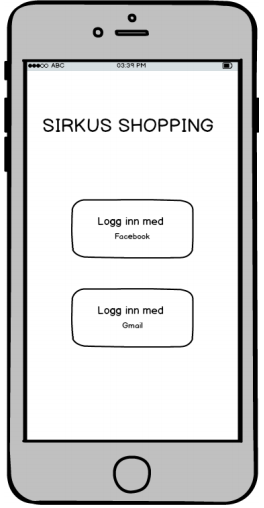
\includegraphics[scale=0.5]{images/prototype1/startskjerm}
\centering %centering the image
\caption{Startskjerm}
\label{fig:startskjerm}
\end{figure}

\noindent I neste trinn får brukeren opp en melding om at dersom hun holder telefonen inntil et produkt kan hun legge det til i handlelisten, vist i Figur \ref{fig:dialogboks}. Ved å trykke “OK” vil boksen lukkes, likt dialogboksene man finner i andre apper.

\begin{figure}[H]
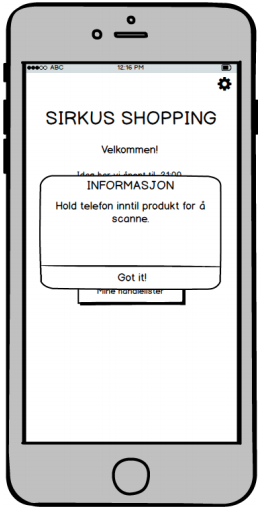
\includegraphics[scale=0.5]{images/prototype1/dialogboks}
\centering %centering the image
\caption{Dialogboks}
\label{fig:dialogboks}
\end{figure}

\noindent For brukere som allerede er logget inn kommer man rett til startsiden. Her ser brukeren logoen til kjøpesenteret, samt informasjon om hvor lenge det holder åpent denne dagen. Brukeren kan velge å lage en ny handleliste, eller å se på eksisterende handlelister. Disse trykkes som knapp. 

\begin{figure}[H]
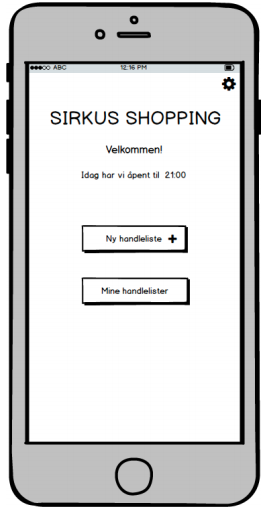
\includegraphics[scale=0.5]{images/prototype1/hjem-skjerm}
\centering %centering the image
\caption{Hjem-skjerm}
\label{fig:hjem-skjerm}
\end{figure}

\noindent Dersom brukeren velger å legge til en ny handleliste må hun skrive inn et navn på handlelisten. Dette gjøres i en dialogboks som kommer opp, og brukeren må bekrefte ved å trykke “OK”. 

\begin{figure}[H]
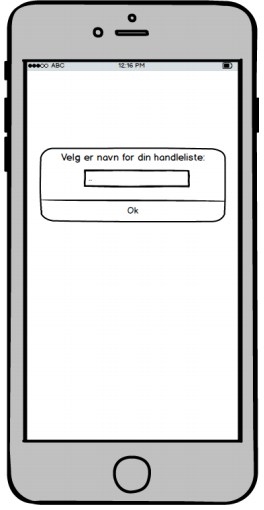
\includegraphics[scale=0.5]{images/prototype1/oppretthandleliste}
\centering %centering the image
\caption{Opprett ny handleliste}
\label{fig:oppretthandleliste}
\end{figure}

\noindent I oversikten “Mine handlelister” kan brukeren se alle handlelistene hun har tilgang til, se Figur \ref{fig:oversikthandlelister} og Figur \ref{fig:oversikthandlelister2}. Det er enten handlelister brukeren har opprettet selv, eller handlelister som andre brukere har delt med vedkommende. På denne siden kan også brukeren legge til flere handlelister ved å trykke på pluss-ikonet. Dette er kjent for brukeren fra andre apper.
\\\\
Nederst på skjermen er det bilde av en søppelbøtte som indikerer at handlelisten kan slettes. Dette gjøres ved å dra handlelisten ned til søppelbøtten. Å bruke søppelbøtte for å slette er et ikon de aller fleste kjenner fra datamaskinen. Å dra elementer til søppelbøtten er også en teknikk man bruker andre steder, som på en datamaskin.

\begin{figure}[H]
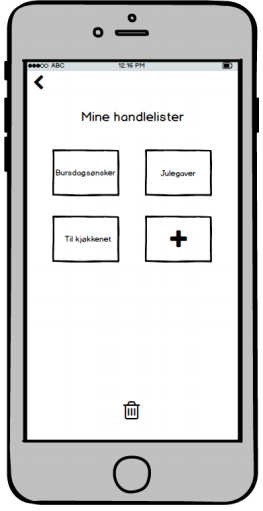
\includegraphics[scale=0.5]{images/prototype1/oversikthandlelister}
\centering %centering the image
\caption{Oversikt over handlelister, variant 1}
\label{fig:oversikthandlelister}
\end{figure}

\begin{figure}[H]
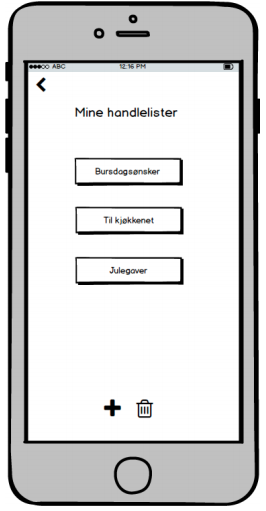
\includegraphics[scale=0.5]{images/prototype1/oversikthandlelister2}
\centering %centering the image
\caption{Oversikt over handlelister, variant 2}
\label{fig:oversikthandlelister2}
\end{figure}

\noindent Når brukeren trykker seg inn på en ønskeliste får vedkommende opp alle varene hun har lagt til i listen. Disse kommer opp med bilde, pris, navn og antall. Det er mulig for brukeren å endre antall av hver vare direkte i listen, eller slette et og et element. Nederst på skjermen kan brukeren se totalsum på varene i listen, og velge å legge alle elementene i listen til i handlekurven.

\begin{figure}[H]
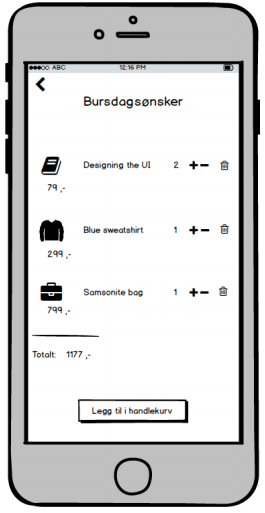
\includegraphics[scale=0.5]{images/prototype1/oversiktliste}
\centering %centering the image
\caption{Oversikt over liste}
\label{fig:oversiktliste}
\end{figure}

Hver vare i handlelisten kan trykkes på for å få opp et mer detaljert skjermbilde av varen. Her er det et stort bilde av varen, pris og størrelse. Varen kan legges til i ønskelisten eller i handlekurven. Dette er det samme skjermbildet som kommer opp når en kunde scanner et produkt med telefonen sin.

\begin{figure}[H]
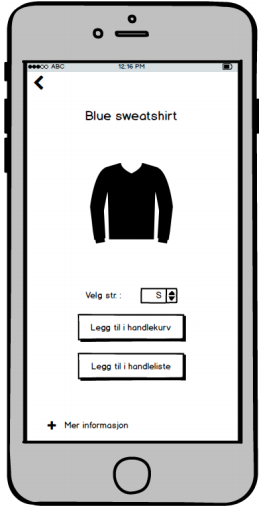
\includegraphics[scale=0.5]{images/prototype1/produkt}
\centering %centering the image
\caption{Visning av produkt}
\label{fig:produkt}
\end{figure}

\noindent Når kunden har fylt opp handlekurven sin med varene hun ønsker kan hun velge å sende ordren. Da vil brukeren få opp et skjermbilde med spørsmål om hun vil betale med Vipps (betalingstjeneste via mobiltelefon) eller om hun vil betale i skranken når hun henter ut varene.

\begin{figure}[H]
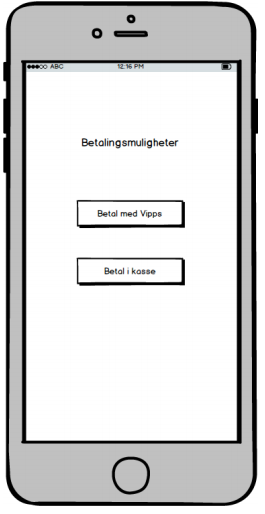
\includegraphics[scale=0.5]{images/prototype1/betalingsmuligheter}
\centering %centering the image
\caption{Betalingsmuligheter}
\label{fig:betalingsmuligheter}
\end{figure}

\noindent Når brukeren har betalt får hun beskjed om hvor lenge det er til hun kan plukke opp varene i varelageret. Dette oppgis i minutter.

\begin{figure}[H]
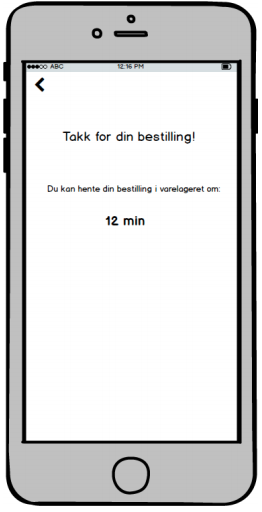
\includegraphics[scale=0.5]{images/prototype1/sluttfortbestilling}
\centering %centering the image
\caption{Sluttført bestilling}
\label{fig:sluttfortbestilling}
\end{figure}

\subsection{Brukertest}
Ved starten av hver test hadde gruppen en sjekkliste som ble gått gjennom før testen startet. Listen var hentet fra forelesningen som omhandlet brukskvalitetstesting\cite{brukskvalitetstesting}. Listen var som følger: 

\begin{enumerate}
    \item Introduser deg selv
    \item Beskriv hensikten med testen
    \item Fortell deltakerne at de kan avbryte når de vil
    \item Beskriv utstyret i rommet og begrensningene til prototypen
    \item Lær bort hvordan man tenker høyt 
    \item Forklar at du ikke kan tilby hjelp under testen
    \item Beskriv oppgaven og introduser produktet
    \item Spør om det er noe de lurer på og kjør testen
    \item Avslutt testen med å la brukeren uttale seg før du samler eventuelle løse tråder
\end{enumerate}

\noindent Mange av disse punktene har den hensikt å gjøre brukeren trygg og komfortabel med testen. Det er viktig å gi brukeren en følelse av kontroll og at han starter testen med en følelse av suksess slik at man får gode og ærlige tilbakemeldinger.
\\\\
Brukeren ble også satt inn i et kort scenario hvor brukeren er på kjøpesenteret for å handle. Siden dette konseptet er ganske annerledes fra en vanlig butikk, ble brukeren satt inn hvordan dette kjøpesenteret fungerte, men gruppen passet på å ikke forklare for mye for at det ikke skulle gå utover testresultatet. Gruppen hadde en genser med en fiktiv strekkode på bordet som testpersonene skulle bruke til oppgavene under testen.

\subsubsection{Testprosedyre}
Papirprototypen ble testet med en test kalt Wizard-of-Oz. Dette er en såkalt low-fidelity prototype-metode\cite[p.~391]{preece}. Den forutsetter at prototypen er basert på software, ettersom brukeren interagerer med softwaren som om han interagerer med produktet. Fordelene med en papirprototype er at den er enkel og billig å lage slik at man kan få tidlig feedback av produktet før man har investert for mye. Siden den er laget av papir og ikke er interaktiv, er det enkelt å forandre designet fort. 
\\\\
Spørsmålene som ble stilt under brukertesten er listet under.

\begin{enumerate}
    \item Du skal lage en oversikt over dine bursdagsønsker. Lista skal hete “bursdagsønsker”.
    \item Du har nå opprettet tre ulike ønskelister. Naviger deg frem til en oversikt over disse.
    \item Legg til en genser i listen over bursdagsønsker. 
    \item Genseren du har lagt i handlelisten er i feil størrelse. Bytt størrelse.
    \item Du vil ikke lenger ha genseren. Fjern genseren.
    \item Du har nå lagt til tre varer til listen og handleturen din er ferdig. Kjøp varene i handlekurven.
    \item Du er på oversikten over dine handlelister. Naviger deg tilbake til startsiden.
    \item Du har fylt opp handlekurven din, men ønsker ikke å kjøpe med én gang. Hva gjør du?
    \item Del genseren med en venn.
\end{enumerate}

\subsubsection{Resultat}
Når man gjennomfører brukertester er det vanlig å gi brukerne et SUS-skjema etter testen. Dette er et skjema for System Usability Scale, og gir brukerne spørsmål om brukervennligheten på en skala fra “sterkt uenig” til “sterkt enig”\cite{usability}. Ut ifra dette kan testerne i ettertid generere en sum som forteller noe om hvor brukervennlig prototypen var. Skalaen går fra 0 til 100, hvor høy sum er best. Alt over 68 regnes som et over gjennomsnittlig resultat.
\\\\
I brukertesten med papirprototypen fikk brukerne i etterkant av testen utdelt et SUS-skjema hvor de svarte på hvor brukervennlig de opplevde prototypen. Resultatene i detalj kan leses i Appendix \ref{App:AppendixB}.
\\\\
Navigasjonsoppgavene og oppretting av lister gikk bra hos alle testdeltakerne. Sletting av genseren var også problemfri. Problemer som gikk igjen hos flere var å forstå forskjellen mellom handlelister og handlekurv, og om de hadde klart å skifte størrelse på genseren fordi det manglet feedback på dette. Det største problemet som alle deltakerne hadde var å få skannet genseren. Man kunne bare ha lagt mobilen inntil genseren så hadde den blitt skannet, men deltakerne letet etter en knapp eller et skjermbilde som viste at appen var klar for skanning. Om deltakerne kom til å skjønne/huske dette ble diskutert i gruppa på forhånd og vi var spente på å se hvordan deltakerne reagerte på dette.

\subsubsection{Analyse}
%-søppelkasseikonet funket
%- la til tab nederst for raskere navigering og for tydeligere skille mellom liste og kurv
%- forandret handleliste til ønskeliste
%- feedback når man skiftet str. Don Norman

Resultatene fra brukbarhetstesten ga gruppen indikasjoner på at noen elementer i prototypen måtte forbedres. Det var ikke alle testpersonene som fikk til oppgavene på tilfredsstillende måte.
\\\\
Når testdeltakerne kom til oppgaven om å legge til en genser i handlekurven, var det mange som ble stille. De skjønte at de skulle skanne strekkoden på genseren, men de ventet på et signal på at det var klart for skanning. Med RFID er mobiltelefonen alltid mottakelig for skanning så man behøver ikke å trykke en plass for å aktivere skanningen, men her hadde designet en mangel på affordance. Det er ingenting som signaliserer at man kan skanne genseren og da tror brukeren at det ikke går ann. 
\\\\
Når man åpnet appen fikk man opp en pop-up som fortalte at man skulle holde telefonen inntil produktet for å skanne. Deltakerne fortalte at de hadde fått med seg denne, men den ble glemt igjen med en gang. Designet her brøt med et av Jacob Nielsens heuristics, recognition rather than recall, som går ut på at brukeren ikke skal behøve å huske informasjon mellom dialoger. Instruksjoner skal være synlige når de trengs\cite[p.~404]{preece}. 
\\\\
Noen av testdeltakerne synes ikke det var helt klart hva forskjellen mellom handlelister og handlekurv var. En grunn til dette var at designet på en handleliste og handlekurven så veldig likt ut, i tillegg til navnene også var veldig like. Poenget med handlelister var at der hadde man varer man ikke skulle kjøpe nå, og at disse listene kunne man dele med andre. Siden man måtte være i butikken for å legge til varer i en liste, passet ikke navnet handleliste. Dette ble derfor forandret til ønskeliste som reflekterte bedre hva som var poenget med listene. 

%norman
%mentale modeller

\subsection{Forbedringer av designet}
%- forandret handleliste til ønskeliste
%- feedback når man skiftet str. Don Norman

Etter å ha gjennomført brukertester bestemte gruppen seg for å utbedre noen ting i designet. Det var flere ting som dukket opp under brukertestene, og gruppen bestemte seg for å endre disse tingene før de gikk videre til neste steg i prosessen.
\\\\
Gruppen fikk tilbakemeldinger om at pop-up vinduet som dukket opp når man logget inn ble trykket “OK” og glemt. Brukerne fikk med andre ord ikke med seg hva som stod i boksen angående scanning av varer. Gruppen valgte derfor å gå bort fra denne løsningen, og gjøre noen endringer på velkomstskjermen. Her ble utseendet og navnet på listene endret, slik at det skulle bli mindre forvirring blant brukerne om hva de ulike elementene var. Ikoner ble lagt til på knappene, slik at brukeren kjenner de igjen senere ved scanning av produkter. 
\\\\
Det ble også lagt til en tab bar nederst på skjermen som hele tiden var synlig, som matchet ikonene på knappene på velkomstskjermen. Dette ble gjort for å forenkle navigeringen i appen siden det var ganske få skjermbilder. Det var å også med på å skille ønskelister fra handlekurv. Når man var på en side, lyste opp det tilhørende ikonet på tab baren for å enklere se hvor man var. 
\\\\
Siden tab baren alltid var synlig ble det mulig å legge til en skann-knapp for brukeren til å trykke på når man skulle skanne en vare. Det var viktig at skann-knappen var synlig hele tiden da brukeren kommer til å skanne varer ofte og man burde slippe å navigere rundt i appen hver gang man skal skanne. 
\\\\
Knappen med “legg til i handlekurv” ble gjort litt større enn knappen med “legg til i ønskeliste” for å få litt mindre fokus på ønskelister siden dette er en valgfri funksjon å bruke. Feltet for “mer informasjon” ble flyttet opp til under bildet av produktet for å vise at det ga informasjon om produktet og ikke om appen. 

%mer her, bilder osv. Bytt ut bildet med et bilde hvor tab baren er med]